\documentclass{article}
\usepackage{tikz}
\usepackage{tikz-qtree}
\usepackage{subfigure}
\usepackage{pgfplots}
\usepackage{float}
\usepackage{graphicx}
\graphicspath{ {./img/} }
\usepackage{subcaption}

\newcommand{\code}[1]{\texttt{#1}}

\title{Evolutionary Audio Synthesis}
\author{Etienne Cella }
\date{June 2018}

\begin{document}

\maketitle

\tableofcontents

\section{Introduction}

\textbf{\textit{Disclaimer: i'm by no means an academic, and this document simply describes an experiment i've been working on in my free time, as part of a learning process. Any comment / criticism is more than welcome.}}\par

\subsection{Context}
I've had a strong interest in electronic music as a teenager, and have now found myself more and more interested by the field of Artificial Intelligence. This experiment gives me an opportunity to combine both these interests, as we'll attempt to build an Evolutionary Audio Synthesis System.\par
We do not \textit{evolve} sounds directly. Rather, we evolve programs that will generate those sounds, that is \textbf{CSound} audio synthesis programs.

\subsection{Tools}

This experiment is written in Python, which we picked because of its elegance, the fast iterations it allows, and the excellent scientific computing libraries it comes with, namely \textbf{numpy} and \textbf{scipy}. For vizualisation, we use the \textbf{matplotlib} and \textbf{graphviz} libraries. We also use the \textbf{CSound} for audio synthesis, we elaborate on this in the next section.

\subsection{Why CSound?}\label{whycsound}
CSound can be thaught of as the assembly of audio synthesis. It is an extremely simple yet powerful language, and its longevity speaks for itself. When describing a signal processing graph, it doesn't get any simpler:

\begin{figure}[H]
    \centering
    \begin{minipage}[b]{.5\textwidth}
        \centering
        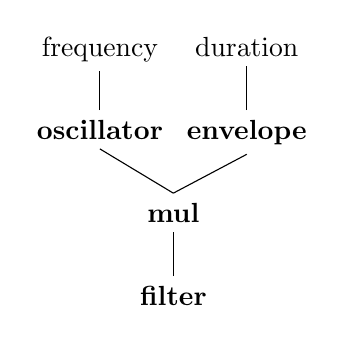
\begin{tikzpicture}[grow'=up]
        \Tree [.\textbf{filter} [.\textbf{mul} [.\textbf{oscillator} frequency ] [.\textbf{envelope} duration ] ]]
        \end{tikzpicture}
        \caption{Signal Processing Graph}
        \label{figtree}
    \end{minipage}%
    \begin{minipage}[b]{.5\textwidth}
        \centering
        \begin{tabular}{ r l l }
    aenv & \textbf{envelope} & duration \\
    aosc & \textbf{oscillator} & frequency \\
    asig & \textbf{mul} & aosc, aenv \\
    out & \textbf{filter} & asig \\
    \end{tabular}
    \caption{CSound implementation}
    \end{minipage}
\end{figure}


\section{Generating Programs}

Generating programs in our case boils down to generating random trees by picking nodes that can be connected together.

\subsection{Variable Types}

When building the tree, we make sure that the input type of the parent node matches the output type of its child. In CSound, types are denoted by the prefixes used for variable names, for example, with \code{asomething}, the type is \code{a}, that is, an audio rate stream.

\subsection{Node Types}

As mentioned, we store programs as trees. These trees are made of nodes, who may hold \textbf{CSound opcodes} (see section \ref{whycsound}) or numerical constants.

In these trees, we'll find three types of nodes, that we'll call \textbf{internal}, \textbf{terminal} and \textbf{constant} nodes. Let's quickly go over these terms:
\begin{itemize}
    \item \textbf{internal node}, a node that holds an opcode whose inputs may be the output of other opcodes
    \item \textbf{terminal node}, a node that holds an opcode whose inputs, if any, are numerical constants
    \item \textbf{constants}, a node holding a numerical constant
\end{itemize}

let's recall figure \ref{figtree}, and vizualise these various node types:

\begin{figure}[H]
    \centering
    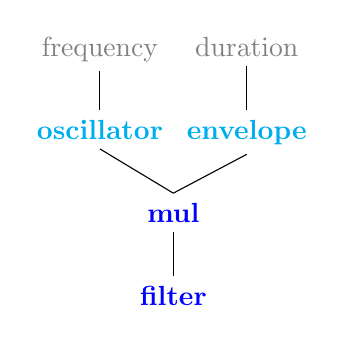
\begin{tikzpicture}[grow'=up]
    \Tree 
        [.\textcolor{blue}{\textbf{filter}}
            [.\textcolor{blue}{\textbf{mul}}
                [.\textcolor{cyan}{\textbf{oscillator}} \textcolor{gray}{frequency} ] 
                [.\textcolor{cyan}{\textbf{envelope}} \textcolor{gray}{duration} ] ]]
    \end{tikzpicture}
    \caption{Node types, \textcolor{blue}{internal}, \textcolor{cyan}{terminal} and \textcolor{gray}{constant}}
\end{figure}%

\subsection{Opcode Signature}

As mentioned in section \ref{introduction}, we have three types of nodes, internal, terminal and constant. Internal and terminal nodes hold CSound opcodes. We have retrieved from CSound's reference the description of a set of nodes that we want to support. Typically in CSound's reference, opcodes are described by their signature, such as: \newline
\code{ares oscil  xamp, xcps, ifn, iphs}\newline
We augment these signature with information helping us to make better educated guesses when picking constants, such as:\newline
\code{ares oscil  xamp:[0,1], xcps:f, ifn:w, iphs:[0,1]} \newline
Here we precise that \textbf{amp} (amplitude) and \textbf{phs} (phase) should be picked in the [0, 1] interval, \textbf{cps} (frequency) is a frequency and \textbf{fn} (function) is a wavetable

\subsection{Opcodes Distribution}\label{distribution}

We support a set of CSound opcodes, some opcodes may appear multiple times with different signatures, think of it as overloads.

The distribution of nodes in the supported set does not reflect their usefulness. For instance, we may have 3 oscillators and 12 envelopes, making the system way more likely to pick an envelope than an oscillator.
We would like the odds of picking an opcode to depend on its functionality and the the functionality of its parent opcode in the tree.

To do so, we associate tags to opcodes, reflecting their functionality, for example, wether it is an envelope, an oscillator, and so on. We then handcraft a matrix storing the probabilities of picking an opcode with a specific tag, given the tag of its parent.

When handcrafting the matrix, what we are doing is try to improve the quality of generated programs by specifying \textit{rules}. For example, \textit{avoid plugging an envelope to the audio output}, or \textit{avoid connecting an envelope output to a reverb}. These rules convey part of the know-how of a sound designer (in a very, very primitive manner). There is a balance to be found between specifying enough rules for the system not to waste too much computation, while preserving enough freedom for the system to come up with surprising solutions.

\section{Evolutionary Program Synthesis}

\subsection{Introduction}\label{introduction}

The goal of the system is to find programs who are good at generating sounds that are \textit{close} to an audioclip selected before the genetic simulation starts. We'll call that audioclip the \textit{target} sound.

Our system evolves programs. During most of this process, programs are stored as trees representing signal processing graphs. Only when generating audio from the programs to evaluate their fitness do we convert them to executable CSound code.

\subsection{Initialization}

We generate an initial population of random programs, constrained by the maximal depth a program may reach and the likelyhood of picking a terminal node (the higher this likelyhood, the less \textit{bushy} the tree will be).

\subsection{Reproduction}

For a predetermined number of generations, we evaluate the fitness of the programs we have, and use the best ones to create the next generation. These offsprings are generated by several methods:
\begin{itemize}
    \item \textbf{exact copy} of their parent
    \item \textbf{mutate constants}, we randomly tweak the numerical constants of the parent, the \textbf{lerp\_factor} parameter lets us control by how much those constants may change
    \item \textbf{subtree mutation}, we pick a node in the parent and append a new random subtree at this node while preserving the overall depth of the tree
    \item \textbf{random generation}, some programs are created randomly, the same way we created the initial population
\end{itemize}

\begin{figure}[H]
\centering
\begin{minipage}{.5\textwidth}
  \centering
  \includegraphics[width=.4\linewidth]{mut_cst_before.png}
  \captionof{figure}{Parent program}
\end{minipage}%
\begin{minipage}{.5\textwidth}
  \centering
  \includegraphics[width=.4\linewidth]{mut_cst_after.png}
  \captionof{figure}{Child program after constant mutation, note that opcodes are preserved while numerical values have changed}
\end{minipage}
\end{figure}

\begin{figure}[H]
\centering
\begin{minipage}{.5\textwidth}
  \centering
  \includegraphics[width=.4\linewidth]{cross_before.png}
  \captionof{figure}{Parent program}
\end{minipage}%
\begin{minipage}{.5\textwidth}
  \centering
  \includegraphics[width=.4\linewidth]{cross_after.png}
  \captionof{figure}{Child program after subtree mutation, note the replacement occured at the \textit{phasor} opcode}
\end{minipage}
\end{figure}

\subsection{Selection}

\subsubsection{Overview}

To evaluate the fitness of programs, we take the following in account:
\begin{itemize}
    \item \textbf{sound similarity}, that is, how close is the spectrum of the sound generated by the program to our \textit{target} sound's spectrum.
    \item \textbf{nodes count}, how much nodes does the tree have. That way we can reward trees with lower nodes count, that is, simpler programs. 
\end{itemize}

\subsubsection{Sound Similarity}

The main goal our system tries to achieve is to produce programs whose output is close to a given audio \textit{target} file.

To evaluate what we'll call \textit{sound similiarity}, we compare the spectrum of the generated audio file with the spectrum of the target file. We define sound similiarity \textbf{s} so that:

\[ \textbf{s} = \sum_{i=1}^{m}\sum_{j=1}^{n}(x_{i,j} - t_{i,j})^2 \]

Each spectrum being an $m\times n$
 matrix, whose axes represent time and frequency, x being the spectrum of the generated sound and t the spectrum of the target sound.

\subsubsection{Preserving Diversity}

By taking multiple factors in account when evaluating fitness, we can preserve diversity within our programs population. Using a single factor, we risk that any \textit{innovation} quickly takes over the whole population, reducing its diversity and lowering the odds of coming up with good solutions by exploring multiple paths simultaneously.

\section{Experimentation}

\subsection{Code Organization}

Our code is organized in the following manner:

\begin{itemize}
  
\item \textbf{analysis}, sound analysis, spectrum computation and comparison

\item \textbf{code\_gen}, CSound code generation from program trees

\item \textbf{csound\_reference}, holds CSound opcodes descriptions

\item \textbf{elements}, tree elements generation based on CSound reference data

\item \textbf{experiment}, glue code between every other elements, responsible for running the overall experiment

\item \textbf{genetic\_operators}, genetic operators used to generate offsprings from trees

\item \textbf{tree}, create and manipulate trees

\item \textbf{util}, miscellaneous utility function

\item \textbf{vizualisation}, vizualise sounds and program trees (using GraphViz for the latter)

\end{itemize}

There also are some test files that are not part of the system itself and are only here to support development.

\subsection{Usage}

To run an experiment, execute the file \code{experiment.py}, experiment parameters are exposed at the bottom of the file. These parameters have the following meaning:

\begin{itemize}
    \item \textbf{file}, the audio file we'll use as a \textit{target} sound
    \item \textbf{intern\_op\_set, term\_op\_set}, opcodes sets, simply returned by \code{read\_op\_set()}
    \item \textbf{num\_generations}, number of generations the simulation will run for
    \item \textbf{init\_population\_size}, the size of the random population generated at the beginning of the simulation
    \item \textbf{selected\_population\_size}, the number of best performing individuals that will be selected from the current generation to create the next one
    \item \textbf{max\_depth} the maximal depth of program trees
    \item \textbf{terminal\_likelyhood}, the probability of picking a terminal opcode when generating a tree, the higher this probability the sparser the trees generated 
    \item \textbf{lerp\_factor}, when using constant mutation, how close do the new numerical values stay from their original values 
    \item \textbf{complexity\_factor}, when evaluating fitness, how much do we reward simpler trees, that is, trees who have a lower node count
    
\end{itemize}

At the end of the experiment, all results will be stored in an \code{output} folder, including:
\begin{itemize}
    \item generated CSound files for the best individual, \code{.orc} and \code{.sco} files.
    \item \code{graphviz} representation of the best individual
    \item audio rendering of the best individual
    \item plot of the best candidates fitness over generations
    \item GIF animation showing the best individuals' graph over generations
\end{itemize}

\subsection{Results}

We'll take a look at an experiment in which the target sound is a clap sampled from a Roland TR-808 drum machine.

We have plotted below the fitness of the best individuals over 512 generations.

\begin{figure}[H]
\includegraphics[width=8cm]{fitness_over_time}
\end{figure}

We observe the curve tends to have a logarithmic shape, as the system makes discoveries and tries to improve on them, making smaller and smaller improvements. We notice that when a significant discovery is made (around generation 100 in the above plot), the \textit{logarithmic pattern} restarts.

We vizualise below the best program after 512 generations:

\begin{figure}[H]
  \centering
  \includegraphics[width=10cm]{graph}
  \caption{Best program after 512 generations}
\end{figure}

Let's compare the waveforms of the target sound and the best generated sound after 512 generations:

\begin{figure}[H]
  \centering
  \includegraphics[width=8cm]{wav_clap_target}
  \caption{Target sound waveform (Roland TR-808 clap)}
\end{figure}

\begin{figure}[H]
  \centering
  \includegraphics[width=8cm]{wav_clap_gen}
  \caption{Best candidate after 512 generations}
\end{figure}

In this selected experiment, the system manages to produce a usable clap sound, close enough to the target sound, within a reasonable amount of generations (of limited size, a couple dozen individuals per generation).

Note that the system has successfully discovered a good strategy for synthesizing clap sounds: apply an envelope on noise generators.

\subsection{Use Cases, Future Developments}

With respect to obtained results and the limits of the computational resources at hand, this system is not aimed at generating audio programs generating sounds similar enough to the target sound to fool the human ear. We're in fact very far from it. But it provides an interesting way to generate new, usable, audio programs, in a supervised way.

As far as future development is concerned, an obvious way to improve the system would be to support more opcodes, and make better educated guesses when building program trees.

We have mentioned in \ref{distribution} that we use a handcrafted matrix to influence the tree building process. We could try to learn this matrix by parsing existing, human-made CSound programs. Or even other programs, say Pure Data or something else, as the tag system is relevant in any audio synthesis environment. We could also try a more radical approach, by updating the weight matrix as the experiment runs, rewarding \textit{good} connections, that is, tag associations that tend to occur in better performing programs. Technically, this would introduce reinforcement learning to the experiment, besides the genetic learning we already have.

\end{document}
